\subsubsection{UC18 - Debug della generazione del \glossario{prompt}}\label{UC18}

\begin{figure}[H]
  \centering
  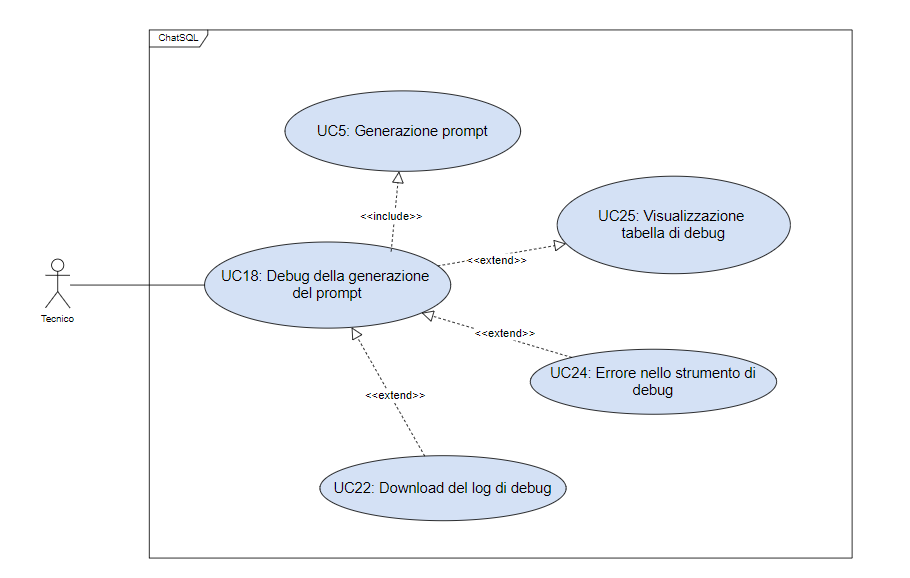
\includegraphics[width=0.90\textwidth]{assets/uc18.png}
  \caption{UC18}
\end{figure}

\paragraph*{Descrizione}
Il Tecnico interroga il sistema per verificare l'interazione tra il \glossario{dizionario dati} e il modello di intelligenza artificiale. Visualizza quindi un file di \glossario{log} contenente il processo di generazione del \glossario{prompt}.

\paragraph*{Attori principali}
Tecnico

\paragraph*{Precondizioni}
\begin{itemize}
  \item L'applicazione è stata avviata con successo;
  \item Il Tecnico ha effettuato correttamente il login (\hyperref[UC1]{UC1});
  \item Il Tecnico ha selezionato l'opzione relativa al \glossario{debug} del sistema;
  \item Il Tecnico ha inserito una richiesta in linguaggio naturale (\hyperref[UC3]{UC3});
  \item Il sistema ha generato un \glossario{prompt} (\hyperref[UC5]{UC5}).
\end{itemize}

\paragraph*{Postcondizioni}
\begin{itemize}
  \item Il tecnico visualizza il file di \glossario{log} generato dal sistema.
\end{itemize}

\paragraph*{Scenario principale}
\begin{enumerate}
  \item Il Tecnico seleziona lo strumento di debug;
  \item Il Tecnico inserisce una richiesta (\hyperref[UC3]{UC3});
  \item Il sistema genera, oltre al prompt (\hyperref[UC5]{UC5}), un file di log che descrive in linguaggio naturale il processo di generazione del prompt stesso; 
\end{enumerate}

\paragraph*{Inclusioni}
\begin{itemize}
  \item Generazione del \glossario{prompt}.
\end{itemize}

\paragraph*{Estensioni}
\begin{itemize}
  \item Errore nella generazione del file di log (\hyperref[UC24]{UC24});
  \item Visualizzazione del contenuto del file di log (\hyperref[UC25]{UC25});
  \item Download del file di log (\hyperref[UC22]{UC22}).
\end{itemize}